\begin{longtable}[]{@{}
  >{\raggedright\arraybackslash}p{(\columnwidth - 2\tabcolsep) * \real{0.3069}}
  >{\raggedright\arraybackslash}p{(\columnwidth - 2\tabcolsep) * \real{0.6931}}@{}}
\toprule\noalign{}
\begin{minipage}[b]{\linewidth}\raggedright
Markdown Syntax
\end{minipage} & \begin{minipage}[b]{\linewidth}\raggedright
Output
\end{minipage} \\
\midrule\noalign{}
\endhead
\bottomrule\noalign{}
\endlastfoot
\# Header 1 & \begin{minipage}[t]{\linewidth}\raggedright
%\chapter*{Chapter}\label{chapter}
{\normalfont\huge\bfseries Chapter} 
\markboth{Chapter}{Chapter}
\end{minipage} \\ \\
\#\# Header 2 & \begin{minipage}[t]{\linewidth}\raggedright
\section*{Section}\label{section}
\markright{Section}
\end{minipage} \\
\#\#\# Header 3 & \begin{minipage}[t]{\linewidth}\raggedright
\subsection*{Subsection}\label{subsection}
\end{minipage} \\
\#\#\#\# Header 4 & \begin{minipage}[t]{\linewidth}\raggedright
\subsubsection*{Subsubsection}\label{subsubsection}
\end{minipage} \\
\#\#\#\#\# Header 5 & \begin{minipage}[t]{\linewidth}\raggedright
{\normalfont\normalsize Paragraph}\label{paragraph}
\end{minipage} \\ \\
\#\#\#\#\#\# Header 6 & \begin{minipage}[t]{\linewidth}\raggedright
{\normalfont\normalsize Subparagraph}\label{subparagraph}
\end{minipage} \\ \\
*italics* & \emph{italics} \\ \\
**bold** & \textbf{bold} \\ \\
superscript\^{}2\^{} & superscript\textsuperscript{2} \\ \\
\textless https://nber.org\textgreater{} & \url{https://nber.org} \\ \\
{[}NBER{]}(https://nber.org) & \href{https://nber.org}{NBER} \\ \\
!{[}caption{]}(monalisa.jpeg) &
\begin{minipage}[t]{\linewidth}\raggedright
\begin{figure}[H]

{\centering 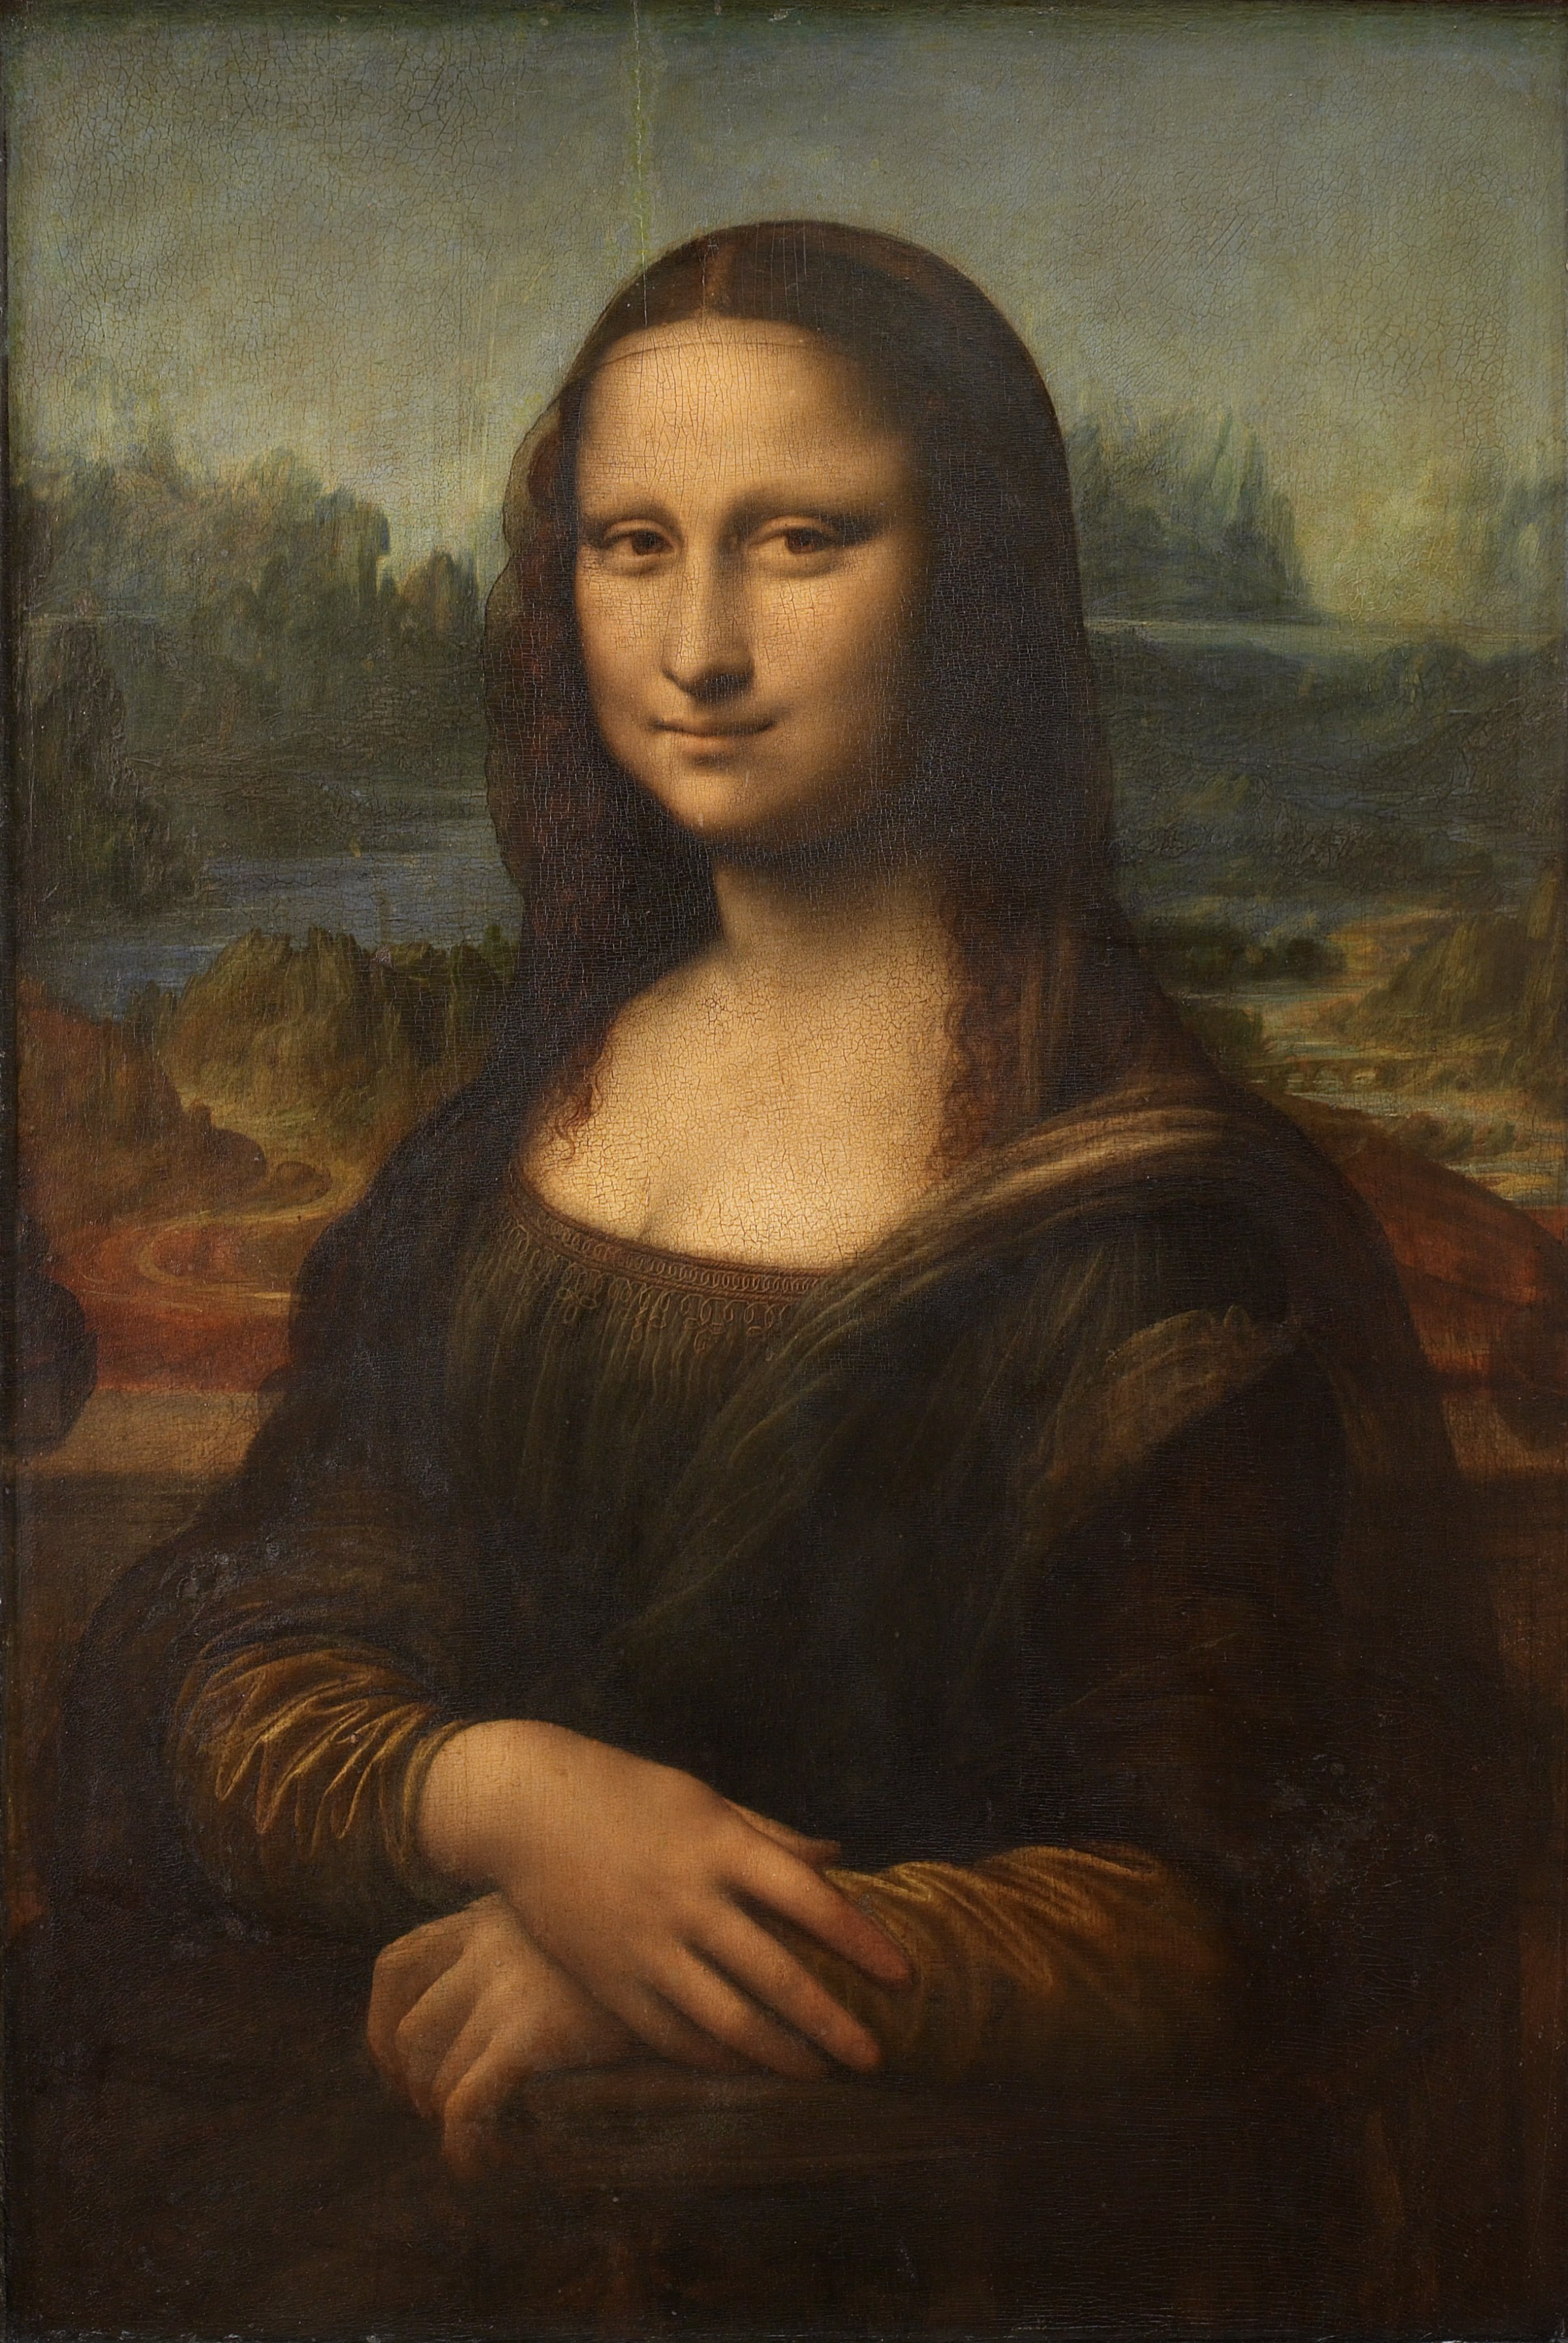
\includegraphics[width=1.39583in]{chapters/images/monalisa.jpeg}}

%\caption{Caption}

\end{figure}%
\end{minipage} \\ \\
unordered list

+ item

\hspace{10pt}- sub-item
    
\hspace{20pt}- sub-sub-item & \begin{minipage}[t]{\linewidth}\raggedright
unordered list

\begin{itemize}
\tightlist
\item
  item
  \begin{itemize}
  \tightlist
  \item
    sub-item
    \begin{itemize}
    \tightlist
    \item
      sub-sub-item
    \end{itemize}
  \end{itemize}
\end{itemize}
\end{minipage} \\ \\
\begin{minipage}[t]{\linewidth}\raggedright
ordered list

1. item

\hspace{10pt}I. sub-item

\hspace{10pt}i. sub-sub-item
\end{minipage} & \begin{minipage}[t]{\linewidth}\raggedright
ordered list\footnote{Use Visual Mode to select your desired style!}

\begin{enumerate}
\def\labelenumi{\arabic{enumi}.}
\item
  item

  \begin{enumerate}
  \def\labelenumii{\Roman{enumii}.}
  \item
    sub-item

    \begin{enumerate}
    \def\labelenumiii{\roman{enumiii}.}
    \tightlist
    \item
      sub-sub-item
    \end{enumerate}
  \end{enumerate}
\end{enumerate}
\end{minipage} \\ \\
inline math: \$E = mc\^{}\{2\}\$ & inline math: \(E = mc^{2}\) \\ \\
display math:

\$\$E = mc\^{}\{2\}\$\$ & \begin{minipage}[t]{\linewidth}\raggedright
display math:\\
\[E = mc^{2}\]\strut
\end{minipage} \\
\end{longtable}
